\appendix
\part*{Appendix}
{
\setlength{\parskip}{-0em}
\startcontents[sections]
\printcontents[sections]{ }{1}{}
}

\label{sec:appendix}

\section{Borader Impacts}
\label{sec::broader}
MetaFind facilitates accessible and coherent 3D scene generation, which can benefit fields like virtual reality, education, and game design. By supporting flexible multimodal queries, it lowers the barrier for non-experts to build rich virtual environments. However, risks include potential misuse in generating misleading content, propagation of bias from training data, and intellectual property concerns tied to retrieved assets. We recommend responsible dataset curation and human oversight to ensure ethical deployment.
\section{Related Work}
3D scene generation serves as the broader task context of our work, encompassing both generative and retrieval-based approaches to assembling realistic virtual environments. Within this paradigm, 3D object retrieval plays a critical role by providing high-quality assets that satisfy semantic, stylistic, and spatial constraints. We first review recent advances in scene generation frameworks, followed by an overview of representative models for multimodal 3D object retrieval.


\subsection{3D Scene Generation Paradigms}

Recent progress in 3D scene generation follows two directions. The first relies on generative models that synthesize entire 3D scenes in mesh, voxel, or neural field formats~\cite{schult2024controlroom3d}. While promising, these methods struggle with ensuring object-level realism or semantic fidelity~\cite{fang2023ctrl}. To address these limitations, a second paradigm emerges that frames scene generation as a layout composition task using retrieved assets from large-scale 3D repositories. LLMs and VLMs exhibit advanced capabilities in various tasks \cite{pan2025evomarlcoevolutionarymultiagentreinforcement,pan2025advevomarlshapinginternalizedsafety,pan2025fairreasonbalancingreasoningsocial}: software engineering \citep{pan2025code,pan2024codevbenchllmsunderstanddevelopercentric}, question answering systems \citep{pan2024chain,pan2024convcoaimprovingopendomainquestion}, and scientific discovery \citep{shao2025sciscigpt}. Methods like LayoutGPT~\cite{feng2023layoutgpt} and I-Design~\cite{ccelen2024design} employ LLMs as planners to generate layouts from text descriptions. More recent techniques, such as LayoutVLM~\cite{sun2024layoutvlm}, improve physical plausibility through differentiable rendering optimization and layout supervision from image-marked datasets. Despite their advances, they still face two fundamental challenges: (1) limited internalized 3D spatial reasoning within VLMs and (2) the inefficiency and poor generalization of supervised fine-tuning, which relies on scarce and imperfect layout annotations. MetaSpatial~\cite{pan2025metaspatial} addresses these issues via a reinforcement learning-based framework that optimizes 3D spatial layouts in real time using physics-aware constraints and rendered-image evaluations. This significantly enhances scene plausibility and coherence.

While MetaSpatial focuses on improving reasoning in layout generation, another crucial but underexplored dimension is the design of the retrieval mechanism itself. Most prior works rely on general-purpose models, such as OpenShape~\cite{liu2023openshape}, to fetch 3D assets. However, these models are not specifically trained for multimodal, scene-conditioned retrieval. They struggle to support arbitrary combinations of user inputs (e.g., missing modality scenarios) and treat object retrieval as an independent parallel process, neglecting layout dependencies. To bridge this gap, we propose a retrieval-centric framework that explicitly incorporates layout context into the retrieval loop. Unlike prior work, our method supports arbitrary modality combinations, performs iterative context-aware retrieval, and introduces a plug-and-play ESSGNN module to encode scene layout as a structured graph. This enables spatially consistent and stylistically coherent scene construction.

\subsection{3D Object Retrieval}
3D object retrieval has traditionally focused on aligning visual and geometric representations of objects with semantic queries in the form of text, image, or point cloud inputs. Early approaches rely on contrastive learning between 2D/3D pairs, such as PointCLIP~\cite{zhang2022pointclip} and CLIP-Forge~\cite{sanghi2022clip}, which repurpose vision-language models for shape retrieval. More recent methods like ULIP~\cite{xue2024ulip} and OpenShape~\cite{liu2023openshape} extend this to tri-modal alignment, embedding text, image, and 3D point clouds into a unified latent space via either single-tower or dual-tower architectures. However, these models are trained purely on object-centric data and assume complete modality availability, limiting their robustness under missing or partial query inputs. Beyond alignment, retrieval models such as SCA3D~\cite{ren2025sca3d} and COM3D~\cite{wu2024com3d} improve representation quality via self-augmentation or compositional reasoning, yet still lack explicit mechanisms to handle arbitrary modality combinations or incorporate contextual cues. OmniBind~\cite{wang2024omnibindlargescaleomnimultimodal} offers more flexible modality binding but is not optimized for retrieval tasks involving spatial constraints. In contrast, MetaFind is explicitly designed for context-aware, multimodal 3D asset retrieval. Our model supports free-form modality combinations and is robust to missing inputs through stochastic masking. Most notably, it augments retrieval with scene context by incorporating an ESSGNN-based layout encoder, enabling iterative, layout-aware asset selection that better supports spatial realism and scene consistency.


\section{Equivariance Proof of ESSGNN - Extension to Semantic Embedding} \label{sec:appendix_equiv_proof}



In this section, we prove that our ESSGNN maintains SE(3) equivariance in 3D space. While the original EGNN \cite{satorras2021n} formulation allows the inclusion of edge features in the message function, these are typically discrete, task-specific features such as bond types or edge labels. In contrast, our ESSGNN introduces edge embeddings \( e_{ij} \) derived from LLM-generated natural language relation descriptions, which are subsequently encoded via a frozen text encoder. Importantly, these semantic edge embeddings are \textit{invariant to the input node positions} \( \rm x \), as they are computed solely from object-level text descriptions and do not depend on spatial coordinates. Therefore, although the semantics encoded in \( e_{ij} \) are richer and more expressive, the mathematical property required for equivariance—the independence of \( e_{ij} \) from \( \rm x \)—remains satisfied. As a result, the message and update equations remain SE(3)-equivariant under our semantic extension, and the original proof structure holds. We now restate and extend the proof below.


Specifically, we show that for any translation vector \( g \in \mathbb{R}^3 \) and any orthogonal transformation \( Q \in \mathbb{R}^{3 \times 3} \), the model satisfies:

\begin{equation}
    Q\rm x^{l+1} + g,\; \rm h^{l+1} = \mathrm{ESSGNN}(Q\rm x^l + g,\; \rm h^l,\; E)
\end{equation}

where \( \rm x^l \) and \( \rm h^l \) are the positions and features of all nodes at layer \( l \), and \( E \) contains edge features including learned semantic embeddings \( e_{ij} \). We begin by assuming that \( \rm h^0 \) is invariant to SE(3) transformations on \( \rm x \), and that semantic edge embeddings \( e_{ij} \) are derived solely from object-level textual descriptions and thus independent of spatial coordinates. Under these assumptions, the edge message computation remains SE(3) invariant. Let us denote the pairwise edge message as:

\begin{equation}
    \rm m_{ij} = \phi_e\left(\rm h_i^l, \rm h_j^l, \| \rm x_i^l - \rm x_j^l \|^2, e_{ij} \right)
\end{equation}
    
Now consider a translation and rotation of all node positions: \( \rm x_i^l \mapsto Q\rm x_i^l + g \). The Euclidean distance term becomes:

\begin{equation}
    \| Q\rm x_i^l + g - (Q\rm x_j^l + g) \|^2 = \| Q(\rm x_i^l - \rm x_j^l) \|^2 = \| \rm x_i^l - \rm x_j^l \|^2
\end{equation}

Hence the edge message is preserved:

\begin{equation}
    \rm m_{ij}' = \phi_e\left(\rm h_i^l, \rm h_j^l, \| Q\rm x_i^l + g - Q\rm x_j^l - g \|^2, e_{ij} \right) = \rm m_{ij}
\end{equation}

The position update in ESSGNN (adapted from EGNN) is defined as:

\begin{equation}
    \rm x_i^{l+1} = \rm x_i^l + \sum_{j \ne i} (\rm x_i^l - \rm x_j^l) \cdot \phi_x(\rm m_{ij})
\end{equation}

We now show that this equation is SE(3) equivariant. Applying the transformation:

\begin{align*}
    Q\rm x_i^l + g + \sum_{j \ne i} \left( Q\rm x_i^l + g - Q\rm x_j^l - g \right) \cdot \phi_x(\rm m_{ij}) &= Q\rm x_i^l + g + Q \sum_{j \ne i} (\rm x_i^l - \rm x_j^l) \cdot \phi_x(\rm m_{ij}) \\
    &= Q \left( \rm x_i^l + \sum_{j \ne i} (\rm x_i^l - \rm x_j^l) \cdot \phi_x(\rm m_{ij}) \right) + g \\
    &= Q\rm x_i^{l+1} + g
\end{align*}

Thus, the coordinate update is SE(3) equivariant.

For the feature update:
\begin{equation}
    \rm h_i^{l+1} = \rm h_i^l + \sum_{j \ne i} \phi_h(\rm m_{ij})
\end{equation}

Since \( \rm m_{ij} \) is invariant to transformations of \( \rm x \), and both \( \rm h_i^l \), \( \rm h_j^l \) and \( e_{ij} \) are independent of the global pose, the feature update is invariant to SE(3) transformations of positions.

Therefore, the ESSGNN update satisfies:

\begin{equation}
    Q\rm x^{l+1} + g,\; \rm h^{l+1} = \mathrm{ESSGNN}(Q\rm x^l + g,\; \rm h^l,\; E)
\end{equation}

This completes the proof that ESSGNN preserves SE(3) equivariance despite the inclusion of semantic edge embeddings. 

\clearpage

\section{Experimental Analysis} \label{sec:experimental analysis}

As shown in Figure~\ref{fig:essgnn_comparison}:

\textbf{Room 1}: Without ESSGNN, the room lacks stylistic coherence—the metallic fireplace and mismatched furniture deviate from the classical theme. With ESSGNN, the scene adopts a unified classical aesthetic with a dark-toned fireplace, matching sofa, and bookshelf.

\textbf{Room 2}: Without ESSGNN, modern office furniture and cluttered seating break the archive theme and hinder functionality. With ESSGNN, compact wooden chairs are arranged around the table, better fitting the aged archive context and improving usability.


\begin{figure*}[h]
  \centering

  \begin{subfigure}[b]{0.45\textwidth}
    \centering
    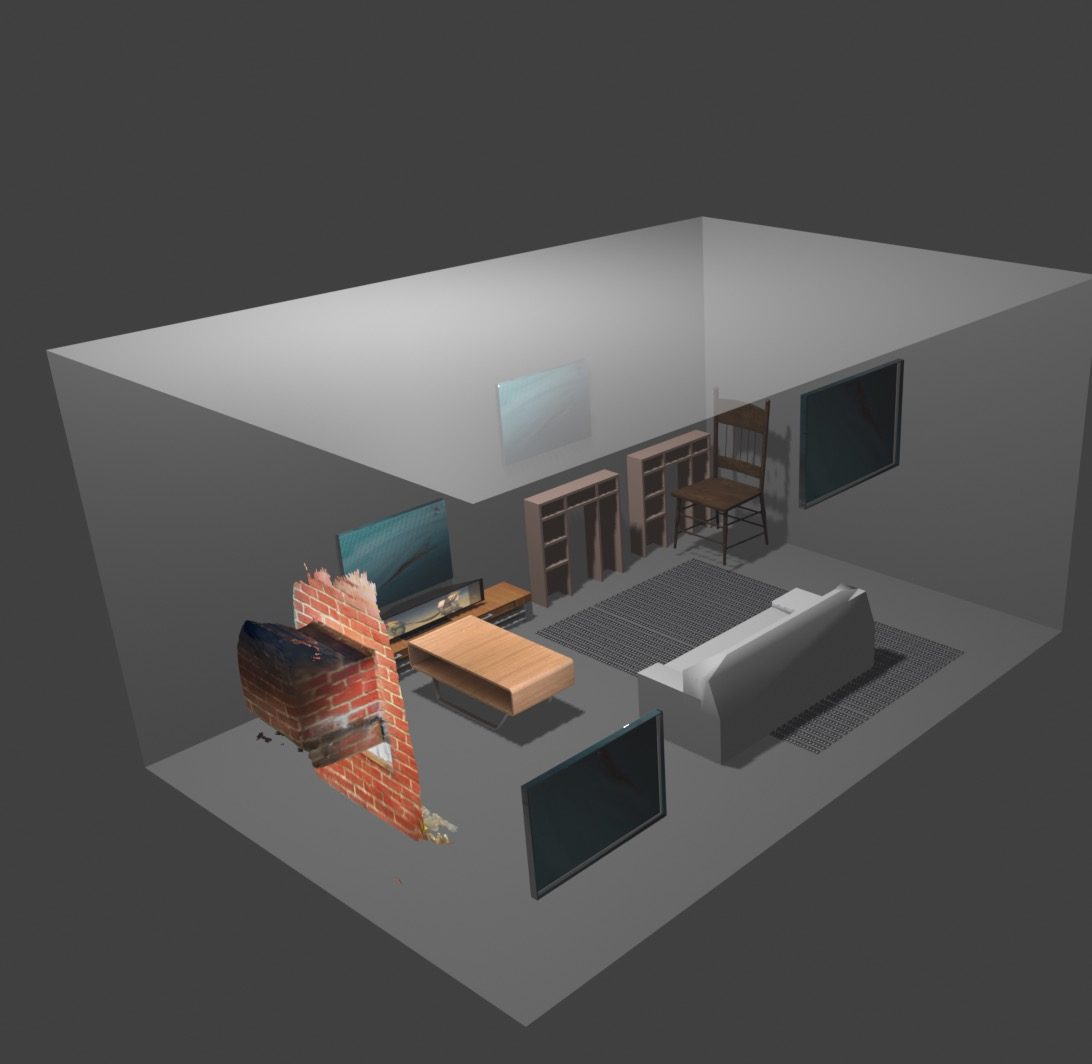
\includegraphics[width=\linewidth]{scene1_no_essgnn.png}
    \caption{Without ESSGNN encoder}
  \end{subfigure}
  \hfill
  \begin{subfigure}[b]{0.45\textwidth}
    \centering
    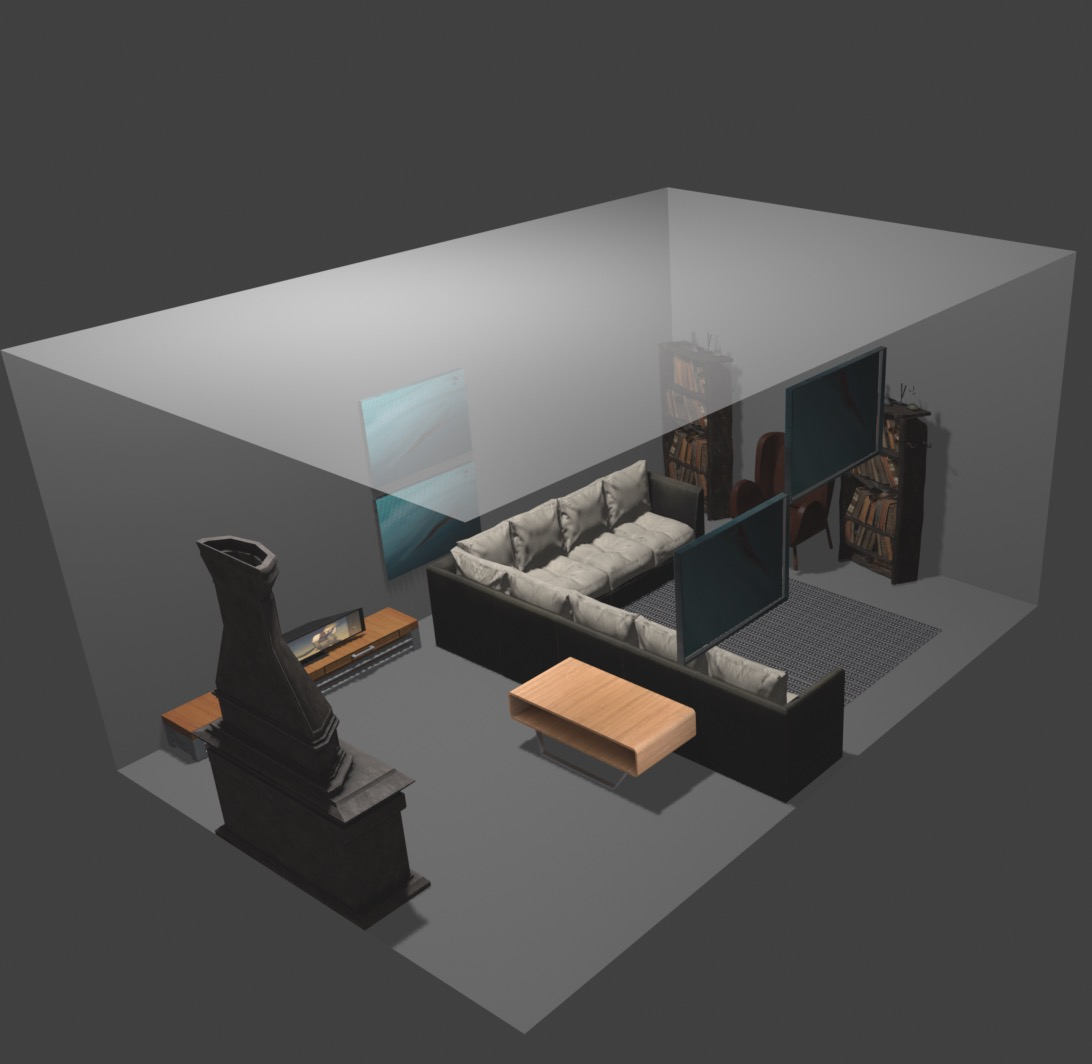
\includegraphics[width=\linewidth]{scene1_with_essgnn.png}
    \caption{With ESSGNN encoder}
  \end{subfigure}

  \vspace{2mm}
  \caption*{\textbf{Room 1 Description:} A classical-style lounge for group leisure and conversation}

  \vspace{5mm}

  \begin{subfigure}[b]{0.45\textwidth}
    \centering
    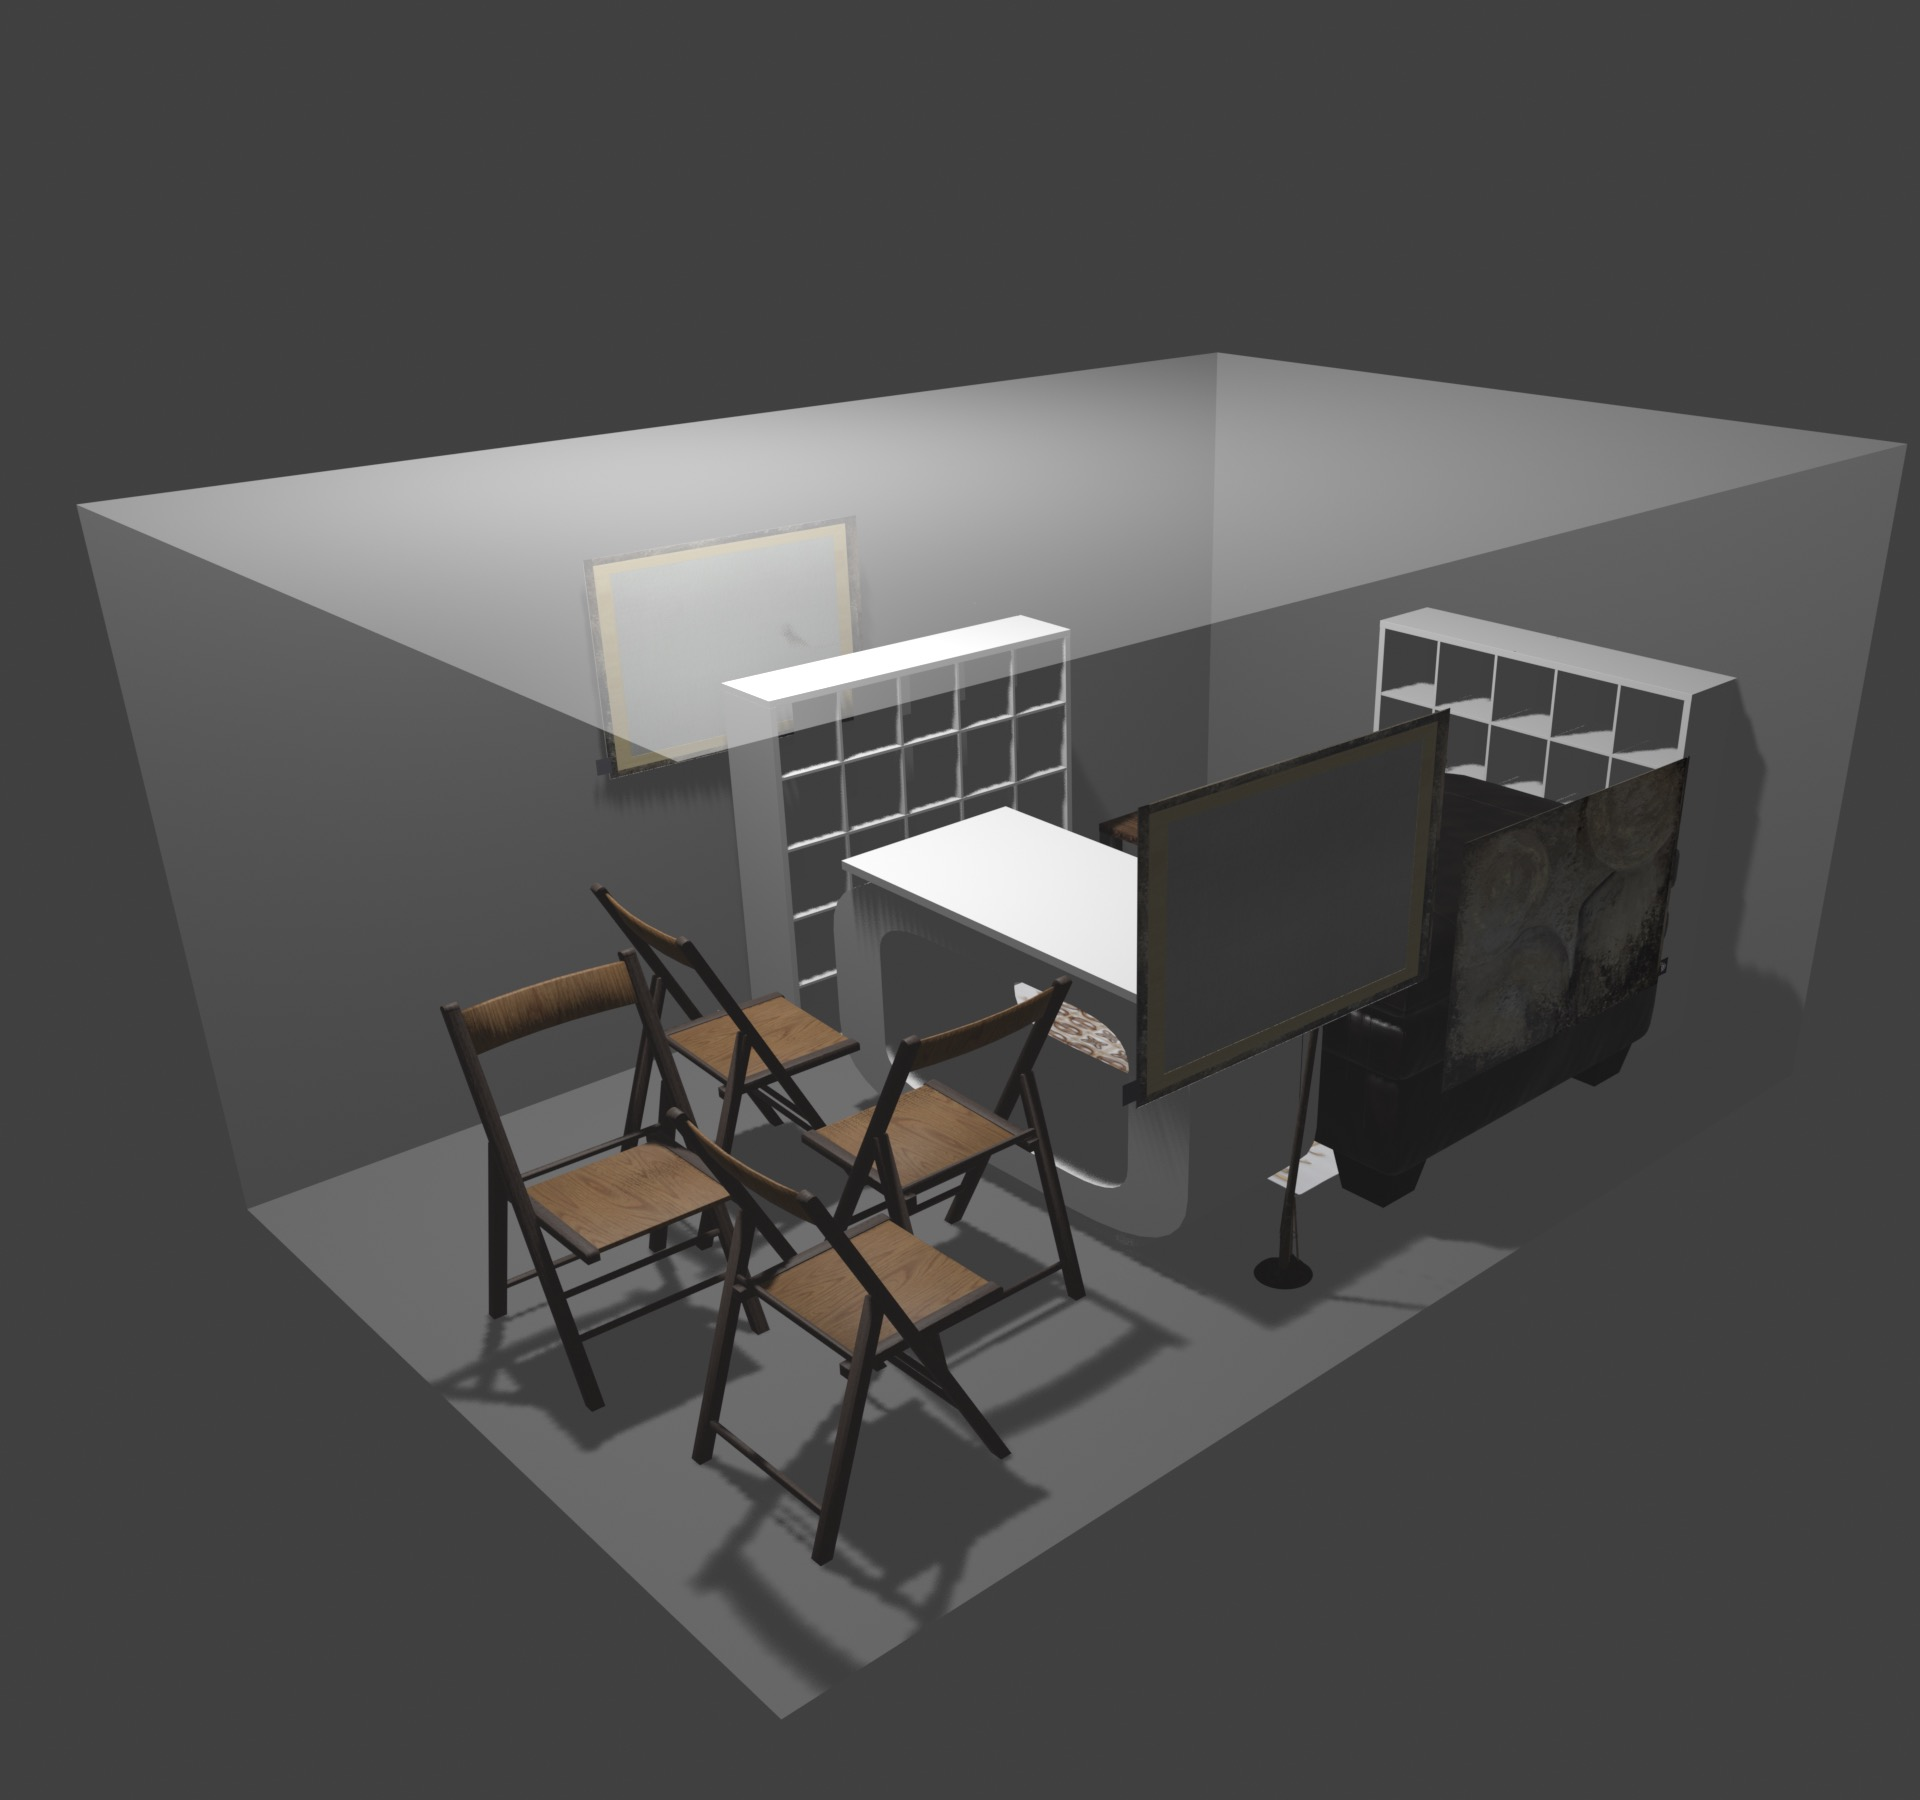
\includegraphics[width=\linewidth]{scene2_no_essgnn.png}
    \caption{Without ESSGNN encoder}
  \end{subfigure}
  \hfill
  \begin{subfigure}[b]{0.45\textwidth}
    \centering
    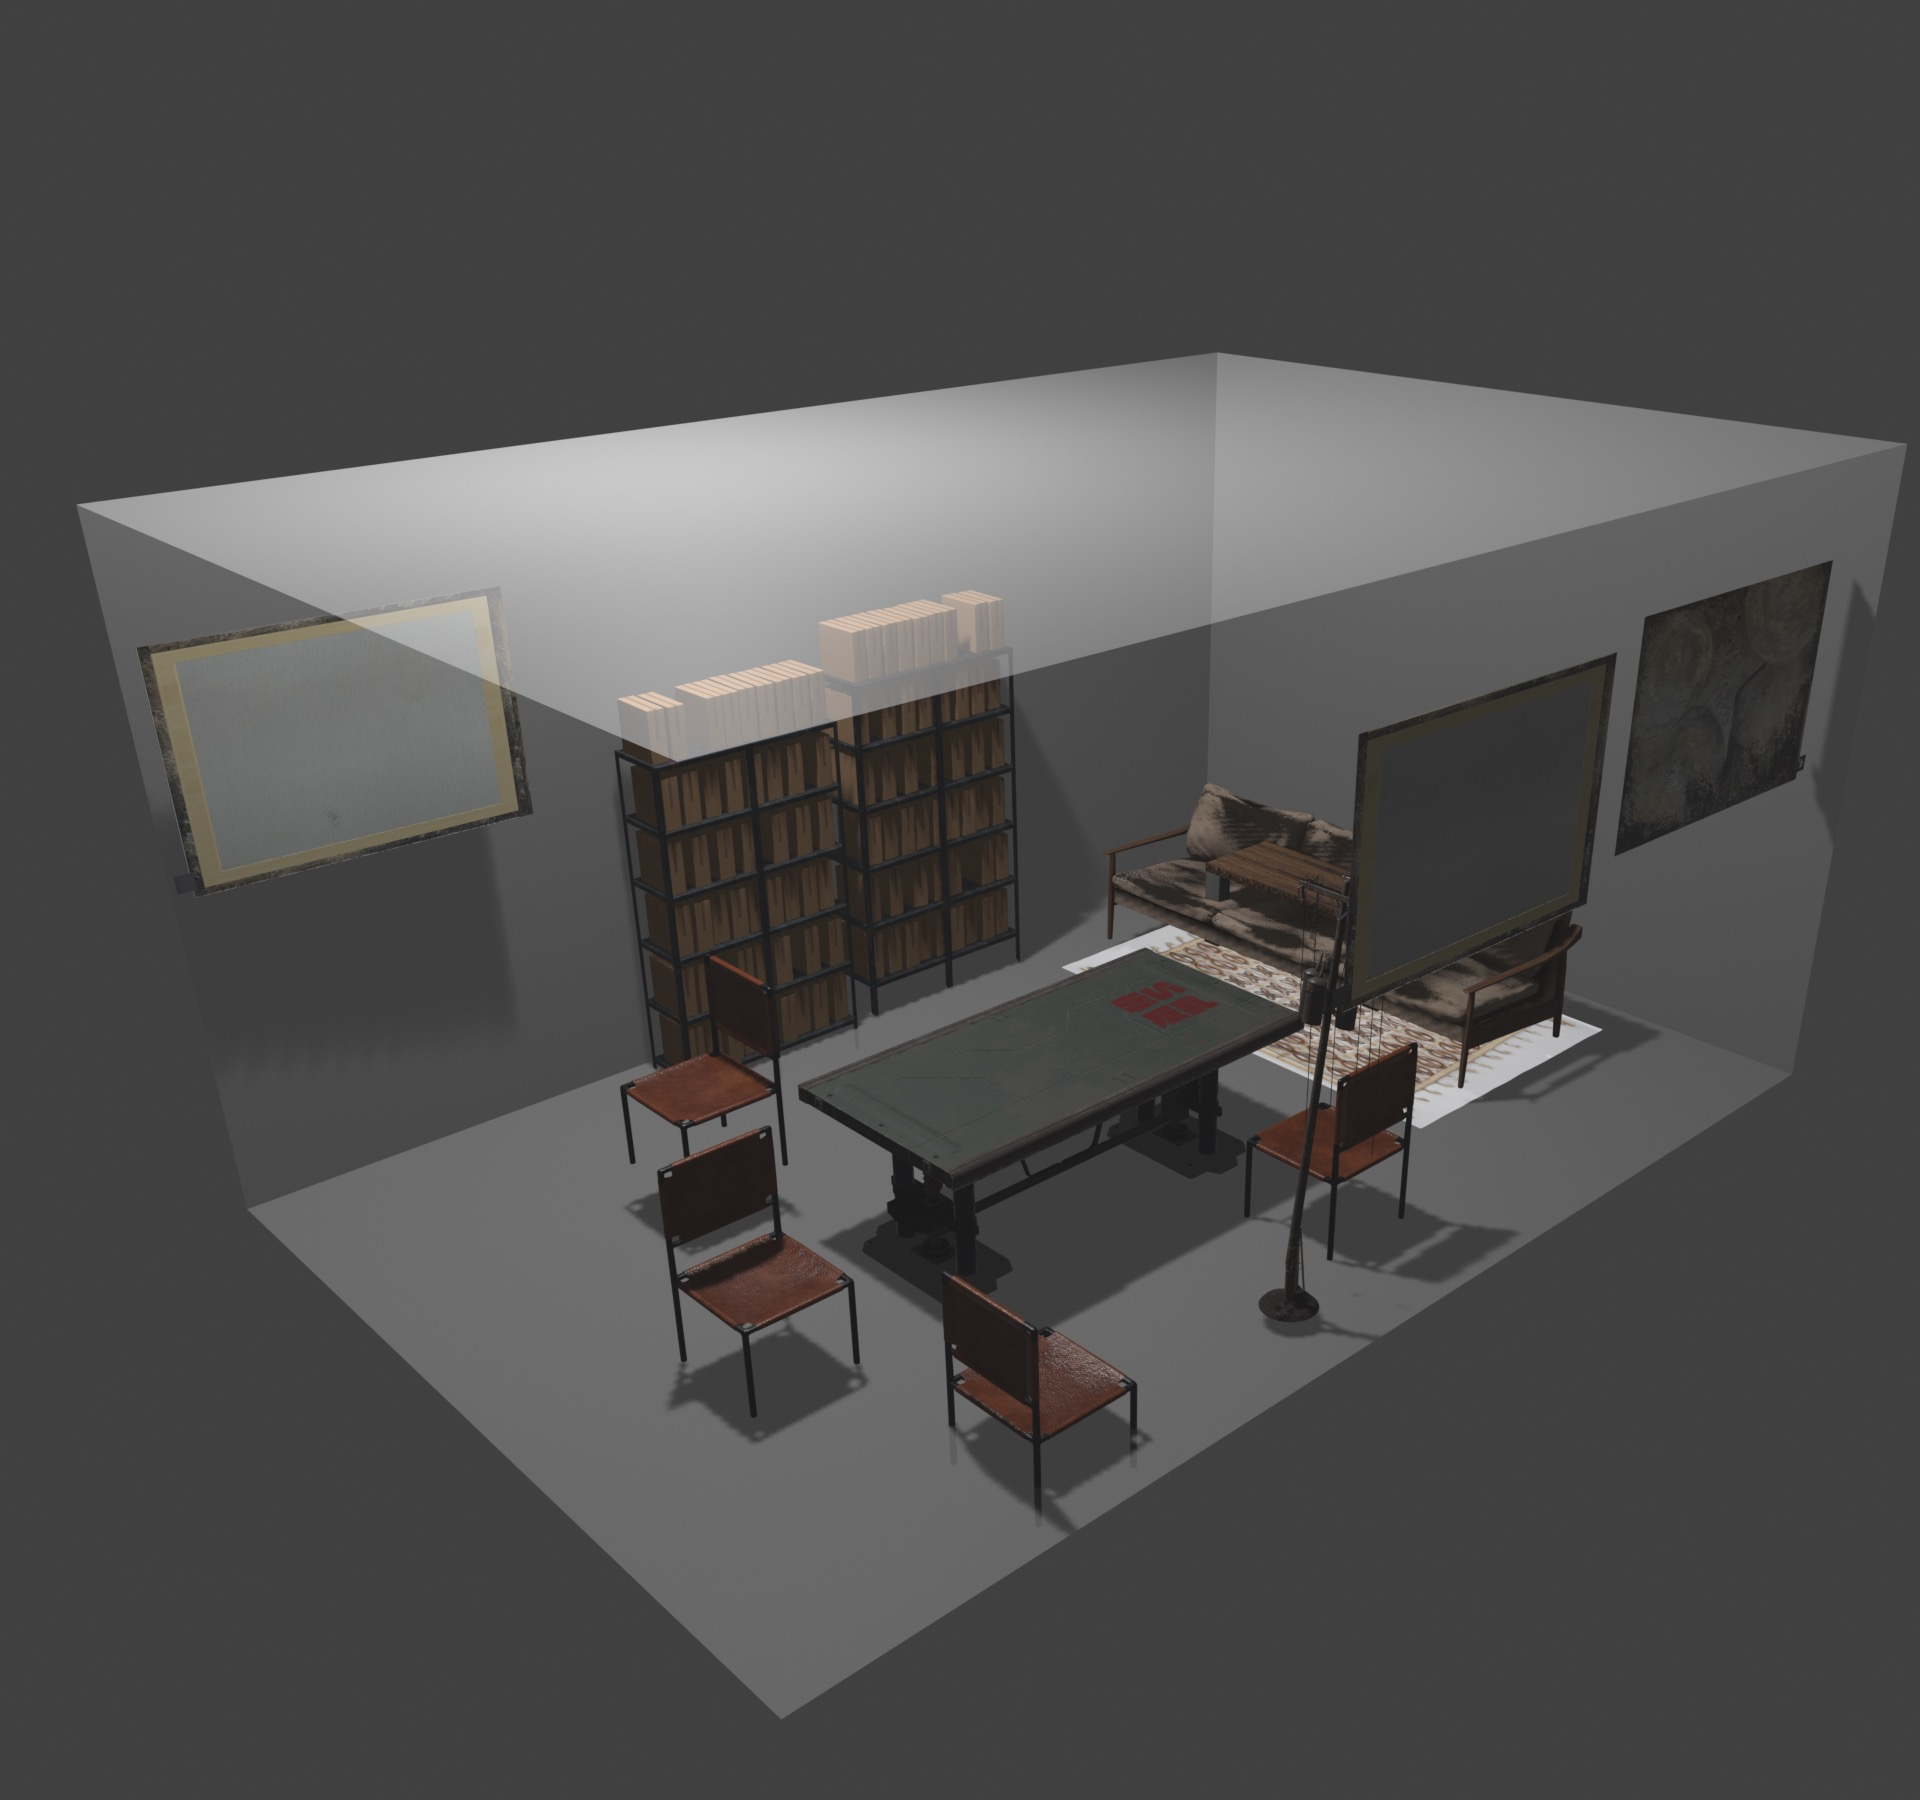
\includegraphics[width=\linewidth]{scene2_with_essgnn.png}
    \caption{With ESSGNN encoder}
  \end{subfigure}

  \vspace{2mm}
  \caption*{\textbf{Room 2 Description:} An aged archive room for research and consultation}

  \caption{Comparison of scene generation with and without ESSGNN encoder.}
  \label{fig:essgnn_comparison}
\end{figure*}